\documentclass[11pt]{article}

\usepackage[margin=0.82in]{geometry}
\usepackage[T1]{fontenc}
\usepackage[utf8]{inputenc}
\usepackage{lmodern}
\usepackage{microtype}
\usepackage{xcolor}
\usepackage{graphicx}
\usepackage{amsmath}
\usepackage{booktabs}
\usepackage{tabularx}
\usepackage{array}
\usepackage{enumitem}
\usepackage{float}
\usepackage[font=small,labelfont=bf,justification=raggedright,singlelinecheck=false]{caption}
\usepackage{hyperref}
\usepackage{tikz}
\usetikzlibrary{arrows.meta, positioning, shapes.geometric, calc, fit, backgrounds}
\graphicspath{{research/robotic_lab_automation_market_2026/figures/}{../research/robotic_lab_automation_market_2026/figures/}}

\definecolor{Ink}{HTML}{16212B}
\definecolor{Muted}{HTML}{5D6B73}
\definecolor{Blue}{HTML}{2563EB}
\definecolor{Teal}{HTML}{0F766E}
\definecolor{Green}{HTML}{15803D}
\definecolor{Amber}{HTML}{B7791F}
\definecolor{Red}{HTML}{B91C1C}
\definecolor{Panel}{HTML}{F5F7FA}
\definecolor{Line}{HTML}{CAD5E2}
\definecolor{SoftBlue}{HTML}{DBEAFE}
\definecolor{SoftTeal}{HTML}{CCFBF1}
\definecolor{SoftGreen}{HTML}{DCFCE7}
\definecolor{SoftAmber}{HTML}{FEF3C7}
\definecolor{SoftRed}{HTML}{FEE2E2}
\definecolor{SoftGray}{HTML}{EDF2F7}

\hypersetup{
  colorlinks=true,
  linkcolor=Blue,
  urlcolor=Teal,
  citecolor=Blue,
  pdftitle={Robotic Laboratory Automation: Market Research, Product Direction, and Execution Roadmap},
  pdfauthor={AgInTiFlow; https://flow.lazying.art}
}

\setlength{\parindent}{0pt}
\setlength{\parskip}{0.56em}
\setlist[itemize]{leftmargin=1.35em, topsep=0.2em, itemsep=0.1em}
\setlist[enumerate]{leftmargin=1.55em, topsep=0.2em, itemsep=0.1em}
\renewcommand{\arraystretch}{1.17}
\raggedbottom

\newcolumntype{Y}{>{\raggedright\arraybackslash}X}
\newcolumntype{L}[1]{>{\raggedright\arraybackslash}p{#1}}
\newcommand{\pill}[2]{%
  \tikz[baseline=(n.base)] \node[rounded corners=2pt, fill=#1, inner xsep=5pt, inner ysep=2pt] (n) {\footnotesize #2};%
}
\newcommand{\artifactroot}{\texttt{research/robotic\_lab\_automation\_market\_2026}}

\title{\vspace{-1.35cm}\textbf{Robotic Laboratory Automation}\\
\large Market Research, Product Direction, and Execution Roadmap}
\author{AgInTiFlow\\\url{https://flow.lazying.art}}
\date{June 5, 2026}

\begin{document}
\maketitle
\vspace{-0.8em}

\begin{abstract}
Robotic laboratory automation is a real market opportunity, but the winning product is unlikely to be a general humanoid laboratory worker. The strongest commercial direction is a constrained, experiment-aware robotic workcell that automates a valuable recurring workflow and converts every run into standardized, auditable data. Public market estimates place global lab automation at USD 8.27 billion in 2024 and USD 18.39 billion in 2033, laboratory robotics at USD 2.353 billion in 2023 and USD 3.864 billion in 2030, and drug discovery services at USD 14.89 billion in 2024 and USD 27.23 billion in 2030. The opportunity is therefore not only labor saving. It is a data, reproducibility, and throughput opportunity in discovery, sample preparation, assay execution, imaging, and later regulated manufacturing.
\end{abstract}

\section{Research Conclusion}

The market is large enough to justify a serious company, but it is also crowded enough that a new entrant should avoid selling a bare robotic arm, a bare hand, or a generic ``AI scientist'' claim. The practical wedge is a robotic assay or sample-preparation workcell that handles a narrow family of protocols with strong data capture, quality control, and repeatability.

\textbf{Best initial direction.} Build a fixed or semi-mobile robotic workcell for screening, sample preparation, imaging-ready assays, and routine biological maintenance. The first product should be judged by completed protocol runs, structured metadata, exception rate, contamination rate, operator hours removed, and customer payback.

\textbf{Avoid as first wedge.} Fully general bench assistance, humanoid locomotion, open-ended tissue manipulation, and regulated cell-therapy manufacturing should not be the first commercial target. These areas are important later, but they create too much integration and validation burden before the core workcell is proven.

\textbf{Strategic thesis.} Existing liquid handlers are strong at pipetting. Enterprise orchestration platforms are strong at scheduling and instrument integration. Custom integrators are strong at bespoke systems. The new entrant's room is between these categories: a repeatable robotic workcell that combines physical manipulation, protocol execution, provenance, and experiment-level learning loops.

\begin{figure}[htbp]
\centering
\includegraphics[width=\linewidth]{experiment_aware_workcell_loop.png}
\caption{Experiment-aware workcell loop. The product loop links protocol definition, robotic execution, QC/provenance, data products, and learning feedback.}
\label{fig:workcell-loop}
\end{figure}

\begin{figure}[htbp]
\centering
\resizebox{\linewidth}{!}{%
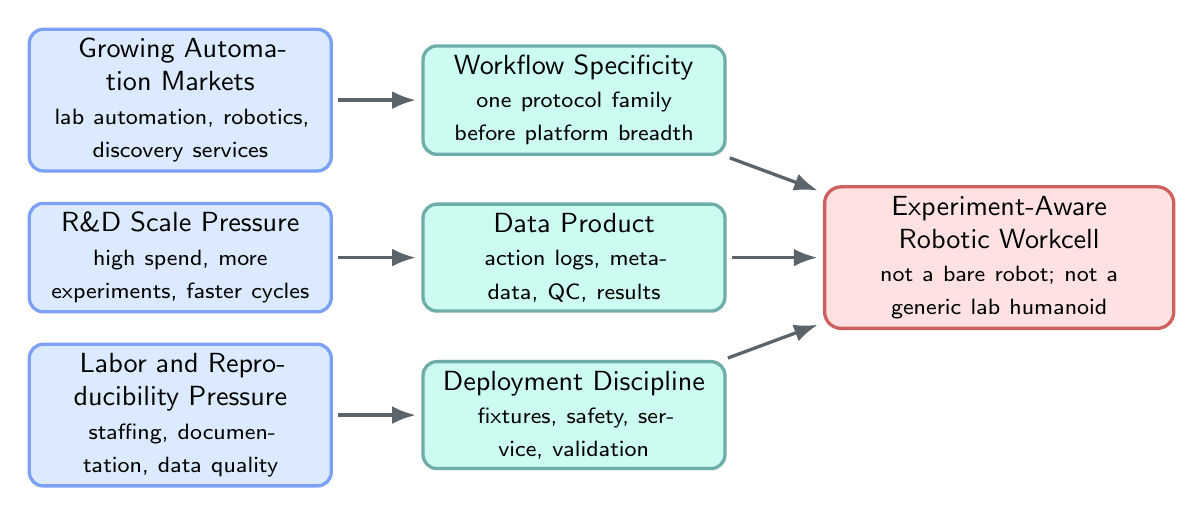
\begin{tikzpicture}[
  font=\sffamily,
  box/.style={rounded corners=5pt, draw=Line, very thick, align=center, minimum height=1.02cm, text width=3.6cm, fill=white},
  driver/.style={box, fill=SoftBlue, draw=Blue!60},
  need/.style={box, fill=SoftTeal, draw=Teal!60},
  wedge/.style={rounded corners=6pt, draw=Red!70, very thick, fill=SoftRed, align=center, minimum height=1.2cm, text width=4.2cm},
  arrow/.style={-{Latex[length=3mm]}, very thick, draw=Ink!70, shorten >=2pt, shorten <=2pt}
]
\node[driver] (market) at (0,2.0) {Growing Automation Markets\\\footnotesize lab automation, robotics, discovery services};
\node[driver] (rd) at (0,0) {R\&D Scale Pressure\\\footnotesize high spend, more experiments, faster cycles};
\node[driver] (labor) at (0,-2.0) {Labor and Reproducibility Pressure\\\footnotesize staffing, documentation, data quality};

\node[need] (workflow) at (5.0,2.0) {Workflow Specificity\\\footnotesize one protocol family before platform breadth};
\node[need] (data) at (5.0,0) {Data Product\\\footnotesize action logs, metadata, QC, results};
\node[need] (deployment) at (5.0,-2.0) {Deployment Discipline\\\footnotesize fixtures, safety, service, validation};

\node[wedge] (product) at (10.4,0) {Experiment-Aware Robotic Workcell\\\footnotesize not a bare robot; not a generic lab humanoid};

\draw[arrow] (market) -- (workflow);
\draw[arrow] (rd) -- (data);
\draw[arrow] (labor) -- (deployment);
\draw[arrow] (workflow) -- (product);
\draw[arrow] (data) -- (product);
\draw[arrow] (deployment) -- (product);
\end{tikzpicture}}
\caption{The investable opportunity is created by the combination of growing automation budgets, R\&D throughput pressure, labor constraints, and reproducibility demands.}
\label{fig:thesis-map}
\end{figure}

\section{Market Sizing}

The direct market should be framed as three adjacent pools rather than one headline number: lab automation systems, laboratory robotics, and outsourced discovery services. The fourth context market is global pharmaceutical sales, which is not a robotics TAM but explains why discovery productivity and cycle time remain valuable.

\begin{table}[htbp]
\centering
\small
\begin{tabularx}{\linewidth}{@{}L{2.65cm}L{1.3cm}L{2.25cm}L{2.35cm}L{1.2cm}Y@{}}
\toprule
\textbf{Market} & \textbf{Scope} & \textbf{Base} & \textbf{Forecast} & \textbf{CAGR} & \textbf{Use in strategy} \\
\midrule
Lab automation & Global & USD 8.27B in 2024 & USD 18.39B in 2033 & 9.27\% & Direct system budget pool for automated laboratories. \\
Laboratory robotics & Global & USD 2.353B in 2023 & USD 3.864B in 2030 & 7.10\% & Narrower robotics subset and closest comparable category. \\
Drug discovery services & Global & USD 14.89B in 2024 & USD 27.23B in 2030 & 10.70\% & Services pool that can be attacked by automated data-generation offerings. \\
Prescription drug sales & Global & Not used as TAM & Above USD 1.7T in 2030 & 7.70\% & Macro demand context for discovery productivity and patent-cliff pressure. \\
\bottomrule
\end{tabularx}
\caption{Market estimates used in the analysis. Raw data are saved in \texttt{data/market\_estimates.csv}.}
\label{tab:market-size}
\end{table}

\begin{figure}[htbp]
\centering
\includegraphics[width=\linewidth]{market_growth_projection.png}
\caption{Comparable market growth pools. The plotted lines use the reported base value, forecast value, and CAGR saved in the research dataset.}
\label{fig:market-growth}
\end{figure}

\textbf{Interpretation.} The direct robotics market is smaller than the broader lab-automation market, but the faster and larger adjacent pool is discovery services. This matters for business model design: a company can begin as a paid workflow or data-generation service, then productize the repeatable workcell once deployment mechanics are understood.

\textbf{Implication for product focus.} A robotics company should not present itself as a generic capital-equipment vendor. It should present itself as a way to produce validated experimental throughput and reusable data assets. This is a stronger value proposition for pharma discovery teams, CROs, and core facilities than hardware novelty.

\section{Demand Drivers}

\subsection{R\&D Scale and Throughput Pressure}

PhRMA member R\&D spending reached USD 104.344 billion in 2024 in the public survey data used here. The year-to-year pattern is not smooth, but the absolute level shows that discovery and development organizations have enough spend to pay for tools that improve throughput, data completeness, or reproducibility.

\begin{figure}[htbp]
\centering
\includegraphics[width=\linewidth]{phrma_rd_spend.png}
\caption{PhRMA member R\&D spend, split into domestic and abroad components. Values are converted from USD millions to USD billions in the plotted artifact.}
\label{fig:phrma-rd}
\end{figure}

\subsection{Workforce and Operations Pressure}

The U.S. Bureau of Labor Statistics reports 351,200 clinical laboratory technologist and technician jobs in 2024, projected employment of 357,200 in 2034, and 22,600 projected annual openings. For automation strategy, the important point is not that robots replace all technicians. The important point is that staffing, repetitive work, documentation, and night/weekend operation create operational pain that automation can address.

\begin{table}[htbp]
\centering
\small
\begin{tabularx}{\linewidth}{@{}L{4.0cm}rL{2.0cm}Y@{}}
\toprule
\textbf{Metric} & \textbf{Value} & \textbf{Period} & \textbf{Strategic reading} \\
\midrule
Median annual wage & USD 61,890 & May 2024 & Labor savings alone can support some use cases, but high-value discovery throughput is usually a stronger ROI story. \\
Employment & 351,200 workers & 2024 & Labs are a large operational environment, but not every lab is an ideal first customer. \\
Projected employment & 357,200 workers & 2034 & Slow growth suggests pressure to do more work per person. \\
Projected annual openings & 22,600 openings/year & 2024--2034 & Replacement hiring and training burden can make automation attractive for repetitive protocols. \\
\bottomrule
\end{tabularx}
\caption{Workforce constraints used in the analysis. Raw data are saved in \texttt{data/workforce\_constraints.csv}.}
\label{tab:workforce}
\end{table}

\subsection{Reproducibility, Provenance, and Data Pressure}

Research institutions and funders increasingly care about replication, reproducibility, data sharing, and standardized records. This shifts the value proposition from ``robot saves labor'' to ``robot produces a complete experimental record.'' In practice, this means a product must log reagent lots, plate maps, actions, deviations, instrument settings, environmental state, image/readout files, QC flags, and operator interventions.

Self-driving-laboratory literature also warns that autonomy is not a generic capability that transfers automatically across every experimental space. Useful systems need measurable task definitions, safety boundaries, and metrics. A marketable workcell should therefore expose a conservative control surface: validated primitives, protocol manifests, audit logs, and exception handling before broad claims of autonomy.

\section{Competitive Landscape}

The public landscape separates into five useful categories.

\begin{table}[htbp]
\centering
\scriptsize
\begin{tabularx}{\linewidth}{@{}L{2.3cm}L{2.8cm}Y Y@{}}
\toprule
\textbf{Company} & \textbf{Category} & \textbf{Public positioning signal} & \textbf{Strategic implication} \\
\midrule
Opentrons Flex & Accessible liquid-handling robot & Public pages emphasize modular pipetting, gripper, deck modules, open-source software/API, and starting configurations around USD 26,400. & Sets the low-cost benchmark. A new entrant should not compete as another pipettor. \\
Automata LINQ & Integrated workcell and cloud orchestration & Public pages emphasize workflow canvas, scheduling, error handling, many instruments, and dense vertical lab layouts. & Shows demand for orchestrated workflows in human-compatible labs. \\
HighRes Cellario OS & Enterprise orchestration & Public pages emphasize digital SOP execution, contextual metadata, APIs, LIMS/ELN integration, and large instrument connectivity. & Data context and enterprise integration matter as much as motion hardware. \\
Multiply Labs & Robotic biomanufacturing cluster & Public pages emphasize closed robotic clusters, GMP-ready operation, sensor logs, and 21 CFR Part 11 compliant records. & Regulated manufacturing is attractive but validation-heavy; enter later. \\
Traditional integrators & Custom automation systems & Bespoke lines around liquid handlers, incubators, readers, hotels, and scheduling software. & New entrant must win on repeatability, faster deployment, protocol portability, or data economics. \\
\bottomrule
\end{tabularx}
\caption{Competitive synthesis from public product pages and category positioning. Raw matrix saved in \texttt{data/competitor\_matrix.csv}.}
\label{tab:competitors}
\end{table}

\begin{figure}[htbp]
\centering
\includegraphics[width=\linewidth]{competitor_positioning.png}
\caption{Directional competitive positioning. Bubble size reflects data-product depth in the saved scoring model; scores are synthesis, not audited market data.}
\label{fig:competitor-positioning}
\end{figure}

\textbf{White space.} The most promising open space is not raw manipulation alone. It is a productized bridge from protocol to physical execution to structured data. The workcell should make protocol runs easier to specify, execute, audit, reproduce, and optimize.

\section{Customer Segmentation}

\begin{table}[htbp]
\centering
\small
\begin{tabularx}{\linewidth}{@{}L{3.0cm}Y Y L{2.7cm}@{}}
\toprule
\textbf{Segment} & \textbf{Pain} & \textbf{What to sell} & \textbf{Priority} \\
\midrule
Biotech discovery teams & Need more assay throughput, consistent runs, and faster design-build-test cycles with limited staff. & Paid pilot workcell or managed automated assay runs with complete metadata package. & \pill{SoftGreen}{High} \\
CROs and discovery-service providers & Backlog, repeatable protocols, customer-facing turnaround time, and margin pressure. & Robotic service cell that increases validated runs per month. & \pill{SoftGreen}{High} \\
Academic core facilities & Repetitive service workflows, scheduling bottlenecks, staff availability, and grant-funded equipment cycles. & Lower-cost pilot cell with shared-service booking and QC reports. & \pill{SoftAmber}{Medium} \\
Synthetic biology and NGS groups & Sample prep and combinatorial workflows already fit automation logic but are vendor crowded. & Differentiated protocol/data layer or specialized manipulation around existing liquid handling. & \pill{SoftAmber}{Medium} \\
Cell therapy and GMP manufacturing & Extremely high process value, but validation, quality systems, and process lock-in are hard. & Later validated module or partnership after discovery workcell maturity. & \pill{SoftRed}{Later} \\
General wet labs & Broad chores and ad hoc handling have weak definition and integration-heavy edge cases. & Avoid as a first product. & \pill{SoftRed}{Low} \\
\bottomrule
\end{tabularx}
\caption{Customer segmentation and recommended priority.}
\label{tab:segments}
\end{table}

\section{Workflow Attractiveness}

The first workflow should be chosen by economics and data value, not by the most impressive robot video. The scoring model below uses five dimensions: automation feasibility, data value, customer pain, regulatory complexity, and a combined near-term score. The underlying data are saved as a CSV artifact.

\begin{figure}[htbp]
\centering
\includegraphics[width=\linewidth]{workflow_attractiveness.png}
\caption{Workflow attractiveness for a first robotic workcell. The strongest initial area is high-feasibility, high-data-value assay and sample-preparation work.}
\label{fig:workflow-attractiveness}
\end{figure}

\begin{table}[htbp]
\centering
\scriptsize
\begin{tabularx}{\linewidth}{@{}L{3.15cm}rrrrY@{}}
\toprule
\textbf{Workflow} & \textbf{Feas.} & \textbf{Data} & \textbf{Pain} & \textbf{Near-term} & \textbf{Interpretation} \\
\midrule
Assay screening and imaging & 4.0 & 4.8 & 4.2 & 4.4 & Best first wedge when the system can connect plate maps, robot actions, readouts, and QC. \\
NGS or sample-prep workcell & 4.4 & 4.1 & 3.8 & 4.2 & Feasible and valuable, but crowded with existing liquid-handling options. \\
Stock-solution preparation and plate dosing & 4.5 & 3.5 & 3.9 & 4.1 & Strong feeder workflow for assays; helps simplify downstream manipulation. \\
Cell-culture media exchange & 4.2 & 3.8 & 4.4 & 4.0 & Repetitive and painful; contamination controls must be designed early. \\
Organoid or tissue maintenance & 2.8 & 4.7 & 4.5 & 3.7 & High value, but biological variability suggests a second-stage product. \\
Cell therapy unit operations & 3.0 & 4.6 & 4.8 & 3.6 & Huge pain and willingness to pay, but validation makes it a later entry point. \\
General bench assistant & 1.8 & 2.5 & 3.0 & 2.0 & Too broad for a first wedge. \\
\bottomrule
\end{tabularx}
\caption{Workflow scoring. Raw data are saved in \texttt{data/workflow\_scores.csv}. Scores are 1--5 directional ratings.}
\label{tab:workflow-scores}
\end{table}

\section{Product Direction}

\subsection{What the Product Should Be}

The recommended product is an \textbf{experiment-aware robotic assay workcell}: a bounded physical cell plus workflow software, protocol manifests, instrument connectors, QC logic, and a structured data layer. It should claim validated operation for a specific protocol family, not broad general intelligence.

\begin{figure}[htbp]
\centering
\resizebox{\linewidth}{!}{%
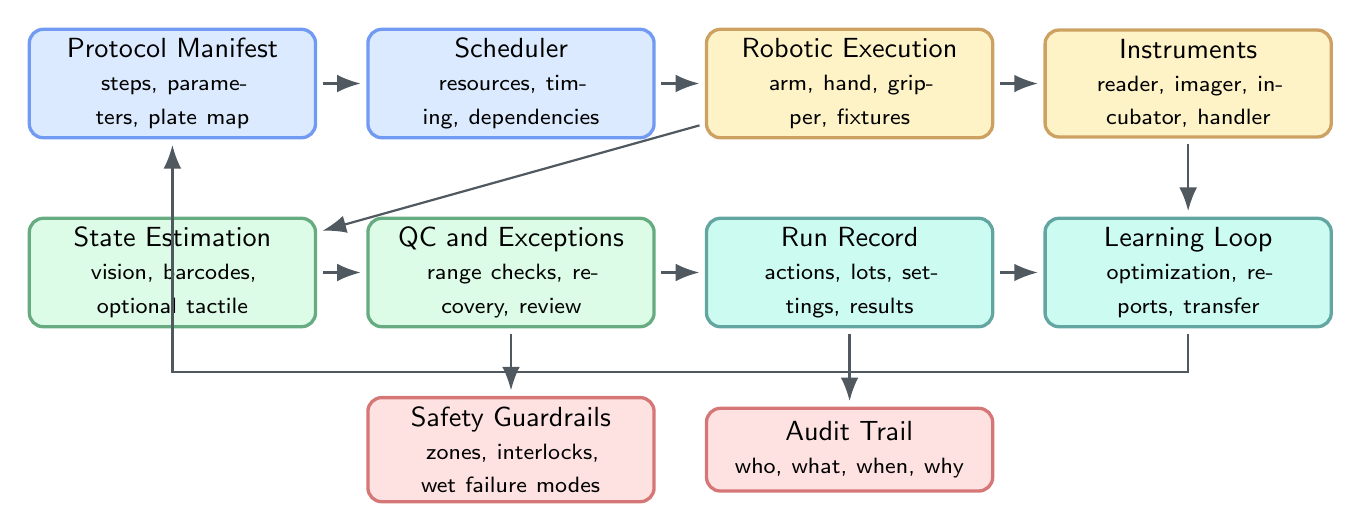
\begin{tikzpicture}[
  font=\sffamily,
  layer/.style={rounded corners=5pt, draw=Line, very thick, fill=white, align=center, minimum height=1.05cm, text width=3.4cm},
  data/.style={layer, fill=SoftTeal, draw=Teal!65},
  control/.style={layer, fill=SoftBlue, draw=Blue!65},
  physical/.style={layer, fill=SoftAmber, draw=Amber!70},
  quality/.style={layer, fill=SoftGreen, draw=Green!65},
  risk/.style={layer, fill=SoftRed, draw=Red!60},
  arrow/.style={-{Latex[length=3mm]}, thick, draw=Ink!75, shorten >=2pt, shorten <=2pt}
]
\node[control] (protocol) at (0,2.4) {Protocol Manifest\\\footnotesize steps, parameters, plate map};
\node[control] (scheduler) at (4.3,2.4) {Scheduler\\\footnotesize resources, timing, dependencies};
\node[physical] (robot) at (8.6,2.4) {Robotic Execution\\\footnotesize arm, hand, gripper, fixtures};
\node[physical] (instruments) at (12.9,2.4) {Instruments\\\footnotesize reader, imager, incubator, handler};

\node[quality] (perception) at (0,0) {State Estimation\\\footnotesize vision, barcodes, optional tactile};
\node[quality] (qc) at (4.3,0) {QC and Exceptions\\\footnotesize range checks, recovery, review};
\node[data] (store) at (8.6,0) {Run Record\\\footnotesize actions, lots, settings, results};
\node[data] (analytics) at (12.9,0) {Learning Loop\\\footnotesize optimization, reports, transfer};

\node[risk] (guard) at (4.3,-2.25) {Safety Guardrails\\\footnotesize zones, interlocks, wet failure modes};
\node[risk] (audit) at (8.6,-2.25) {Audit Trail\\\footnotesize who, what, when, why};

\draw[arrow] (protocol) -- (scheduler);
\draw[arrow] (scheduler) -- (robot);
\draw[arrow] (robot) -- (instruments);
\draw[arrow] (instruments) -- (analytics);
\draw[arrow] (robot) -- (perception);
\draw[arrow] (perception) -- (qc);
\draw[arrow] (qc) -- (store);
\draw[arrow] (store) -- (analytics);
\draw[arrow] (qc) -- (guard);
\draw[arrow] (store) -- (audit);
\draw[arrow] (analytics.south) -- ++(0,-0.55) -| (protocol.south);
\end{tikzpicture}}
\caption{Reference architecture for a productized robotic assay workcell. The core asset is the closed loop from protocol to execution to structured data.}
\label{fig:architecture}
\end{figure}

\subsection{Hardware Direction}

\begin{table}[htbp]
\centering
\small
\begin{tabularx}{\linewidth}{@{}L{3.2cm}YY@{}}
\toprule
\textbf{Decision} & \textbf{Recommended near-term choice} & \textbf{Reasoning} \\
\midrule
Base & Fixed bench cell first; mobile base only when it reduces instrument duplication. & Fixed cells reduce navigation, safety, and validation burden. \\
Manipulator & Arm plus tool-changing gripper/hand, with fixtures that simplify grasping. & The environment should be redesigned around robot-friendly primitives. \\
Dexterous hand & Prototype with simpler grippers and direct-drive hands; reserve tendon-driven designs for repeated contact-rich production tasks. & Dexterity is valuable, but unsupported hand complexity can slow product validation. \\
Vision & Mandatory side/wrist vision plus barcode/label reading. & Visual state checks are needed for reliability, auditability, and exception handling. \\
Tactile sensing & Add only for contact-rich steps such as insertion, cap manipulation, slip detection, or delicate handling. & Tactile feedback is valuable where it changes success probability; otherwise it adds integration load. \\
Environment & Use carriers, racks, fixtures, standardized containers, and plate-based formats. & The cheapest robotics improvement is usually workflow redesign. \\
\bottomrule
\end{tabularx}
\caption{Hardware direction for a first commercial workcell.}
\label{tab:hardware}
\end{table}

\subsection{Software and Data Direction}

The software should be treated as the durable asset. Hardware changes across customers, but protocol representation, instrument connectors, exception taxonomy, metadata schema, and QC reporting can compound.

\begin{itemize}
  \item \textbf{Protocol manifests:} explicit inputs, allowed ranges, timing windows, plate maps, reagent lots, controls, and expected readouts.
  \item \textbf{Execution primitives:} guarded pick, place, pipette, mix, cap, uncap, scan, image, incubate, wait, and recover.
  \item \textbf{Run record:} timestamped actions, robot state, instrument settings, environmental context, operator intervention, and failure mode.
  \item \textbf{Quality layer:} positive/negative controls, plate-level QC, outlier flags, contamination indicators, drift detection, and rerun logic.
  \item \textbf{Customer output:} markdown/PDF run report, machine-readable data package, and reproducibility manifest.
\end{itemize}

\section{Business Model and Pilot Economics}

The safest business model sequence is service-first, then productized deployment.

\begin{enumerate}
  \item \textbf{Design-partner service:} run customer protocols in a controlled internal or partner lab and deliver data packages.
  \item \textbf{Paid pilot cell:} install a bounded workcell for one protocol family with clear exit criteria.
  \item \textbf{Repeatable product:} sell or lease a standardized workcell with support, software, and protocol packages.
  \item \textbf{Workflow network:} reuse protocol definitions, connectors, QC logic, and datasets across customers.
\end{enumerate}

\begin{figure}[htbp]
\centering
\includegraphics[width=\linewidth]{roi_sensitivity.png}
\caption{Illustrative pilot economics. The data are planning assumptions saved in \texttt{data/roi\_scenarios.csv}, not sourced market facts.}
\label{fig:roi}
\end{figure}

\begin{table}[htbp]
\centering
\scriptsize
\begin{tabularx}{\linewidth}{@{}L{2.6cm}r r r rY@{}}
\toprule
\textbf{Scenario} & \textbf{Capex} & \textbf{Annual value} & \textbf{Payback} & \textbf{Extra runs/mo.} & \textbf{Reading} \\
\midrule
Academic core pilot & USD 180k & USD 116k & 24.0 mo. & 12 & Feasible if the project is subsidized by equipment funding or shared-facility utilization. \\
Biotech discovery team & USD 280k & USD 386k & 10.4 mo. & 28 & Attractive first customer when assay throughput is a real bottleneck. \\
CRO service cell & USD 420k & USD 704k & 8.1 mo. & 75 & Strongest payback when validated capacity can be sold or backlog reduced. \\
Regulated manufacturing pilot & USD 650k & USD 670k & 13.0 mo. & 20 & Attractive economics but more difficult validation and quality-system requirements. \\
\bottomrule
\end{tabularx}
\caption{Derived pilot economics. The model combines labor relief, incremental runs, service/software fees, and support assumptions.}
\label{tab:roi}
\end{table}

\section{Regulatory, Quality, and Safety}

For discovery research, the first regulatory burden is usually internal quality, traceability, and data integrity rather than formal manufacturing validation. For clinical, diagnostic, or GMP workflows, the burden changes materially. The FDA Part 11 guidance is relevant because electronic records and signatures must be reliable, but Part 11 compliance alone is not enough; underlying predicate rules and process validation remain important.

\textbf{Practical quality design.}
\begin{itemize}
  \item Keep a complete audit trail for protocol version, operator, robot program, instrument settings, reagent lots, environment, and exception resolution.
  \item Treat every deviation as structured data, not as a free-text afterthought.
  \item Separate research-use workflows from regulated workflows in product claims and documentation.
  \item Define run acceptance criteria before the run starts.
  \item Make safety cases concrete: pinch points, spills, sharps, solvent compatibility, biological contamination, incubator access, and emergency stop behavior.
\end{itemize}

\clearpage
\section{Execution Roadmap}

\begin{figure}[htbp]
\centering
\resizebox{\linewidth}{!}{%
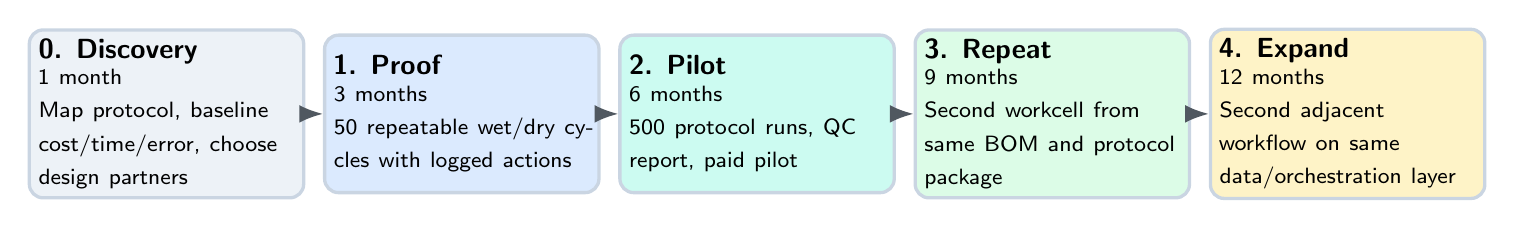
\begin{tikzpicture}[
  font=\sffamily,
  phase/.style={rounded corners=5pt, draw=Line, very thick, align=left, text width=3.25cm, minimum height=2.0cm, fill=white},
  arrow/.style={-{Latex[length=3mm]}, thick, draw=Ink!75}
]
\node[phase, fill=SoftGray] (p0) at (0,0) {\textbf{0. Discovery}\\\footnotesize 1 month\\Map protocol, baseline cost/time/error, choose design partners};
\node[phase, fill=SoftBlue] (p1) at (3.75,0) {\textbf{1. Proof}\\\footnotesize 3 months\\50 repeatable wet/dry cycles with logged actions};
\node[phase, fill=SoftTeal] (p2) at (7.5,0) {\textbf{2. Pilot}\\\footnotesize 6 months\\500 protocol runs, QC report, paid pilot};
\node[phase, fill=SoftGreen] (p3) at (11.25,0) {\textbf{3. Repeat}\\\footnotesize 9 months\\Second workcell from same BOM and protocol package};
\node[phase, fill=SoftAmber] (p4) at (15,0) {\textbf{4. Expand}\\\footnotesize 12 months\\Second adjacent workflow on same data/orchestration layer};
\draw[arrow] (p0) -- (p1);
\draw[arrow] (p1) -- (p2);
\draw[arrow] (p2) -- (p3);
\draw[arrow] (p3) -- (p4);
\end{tikzpicture}}
\caption{Execution roadmap. Detailed KPI data are saved in \texttt{data/roadmap\_kpis.csv}.}
\label{fig:roadmap}
\end{figure}

\begin{table}[htbp]
\centering
\small
\begin{tabularx}{\linewidth}{@{}L{2.6cm}L{2.0cm}YY@{}}
\toprule
\textbf{Phase} & \textbf{Length} & \textbf{Technical exit} & \textbf{Business exit} \\
\midrule
Workflow discovery & 1 month & One protocol mapped into primitives, QC fields, and exceptions. & Two design partners and baseline manual metrics. \\
Benchtop proof & 3 months & 50 repeatable wet/dry cycles without unresolved unsafe states. & Measured improvement in labor time, scheduling, or data completeness. \\
Pilot workcell & 6 months & 500 protocol runs with QC report and recovery playbooks. & Paid pilot or paid data-generation service. \\
Repeatable deployment & 9 months & Second workcell from same bill of materials and protocol package. & Payback under 18 months for one defined segment. \\
Platform expansion & 12 months & Second adjacent workflow without replacing the data layer. & Reusable protocol package or managed service line. \\
\bottomrule
\end{tabularx}
\caption{Milestones and exit criteria.}
\label{tab:roadmap}
\end{table}

\clearpage
\section{Research Artifacts}

All structured research artifacts are saved under \artifactroot. Public-source facts and derived assumptions are separated so future analysis can update either without rewriting the report logic.

\begin{table}[H]
\centering
\small
\begin{tabularx}{\linewidth}{@{}L{5.0cm}Y@{}}
\toprule
\textbf{Artifact} & \textbf{Contents} \\
\midrule
\path{data/market_estimates.csv} & Lab automation, laboratory robotics, drug discovery services, and pharma-sales context estimates. \\
\path{data/phrma_rd_spend_2018_2024.csv} & PhRMA member R\&D spend series used in Figure~\ref{fig:phrma-rd}. \\
\path{data/workforce_constraints.csv} & BLS labor-market metrics used for operational-pressure analysis. \\
\path{data/competitor_matrix.csv} & Public competitor/category synthesis. \\
\path{data/competitor_positioning_scores.csv} & Directional scoring model used in Figure~\ref{fig:competitor-positioning}. \\
\path{data/workflow_scores.csv} & Workflow attractiveness scoring used in Figure~\ref{fig:workflow-attractiveness}. \\
\path{data/roi_scenarios.csv} & Derived pilot-economics assumptions used in Figure~\ref{fig:roi}. \\
\path{data/roadmap_kpis.csv} & Phase plan, technical exits, business exits, and primary risks. \\
\path{data/source_register.csv} & Source IDs, source titles, publishers, access dates, URLs, and key facts used. \\
\path{figures/} & Market, R\&D spend, workflow, competitor, ROI, and workcell-loop figures. \\
\path{notes/research_method.md} & Method notes and separation between sourced facts and derived judgments. \\
\bottomrule
\end{tabularx}
\caption{Saved data and artifact inventory.}
\label{tab:artifacts}
\end{table}

\clearpage
\section{Source Register}

\begin{table}[H]
\centering
\scriptsize
\begin{tabularx}{\linewidth}{@{}L{3.2cm}L{3.8cm}Y@{}}
\toprule
\textbf{Source ID} & \textbf{Source} & \textbf{Key data or idea used} \\
\midrule
\texttt{GVR-AUTO} & Grand View Research, Lab Automation Market & USD 8.27B 2024 market, USD 18.39B 2033 forecast, 9.27\% CAGR. \\
\texttt{GVR-ROBOTICS} & Grand View Research, Laboratory Robotics Market & USD 2.353B 2023 market, USD 3.864B 2030 forecast, 7.1\% CAGR. \\
\texttt{MNM-DDS} & MarketsandMarkets via PR Newswire & Drug discovery services market USD 14.89B in 2024, USD 27.23B in 2030, 10.7\% CAGR. \\
\texttt{PHRMA} & PhRMA annual membership survey & Member R\&D spend, including USD 104.344B total in 2024. \\
\texttt{BLS-LAB} & U.S. Bureau of Labor Statistics & Clinical lab technologist/technician wage, employment, projection, and openings. \\
\texttt{EVALUATE} & Evaluate World Preview release & Global prescription drug sales forecast above USD 1.7T by 2030. \\
\texttt{OPENTRONS} & Opentrons Flex public page & Price and positioning signals for low-cost liquid-handling automation. \\
\texttt{AUTOMATA} & Automata LINQ public pages & Cloud workflow creation, scheduling, error handling, instrument breadth, dense layouts. \\
\texttt{HIGHRES} & HighRes Cellario public pages & Orchestration, metadata, digital SOPs, APIs, and instrument connectivity. \\
\texttt{MULTIPLY} & Multiply Labs public page & GMP-ready robotic manufacturing cluster positioning and data-record claims. \\
\texttt{FDA-PART11} & U.S. FDA Part 11 guidance & Electronic-record scope and reminder that predicate-rule compliance remains required. \\
\texttt{SDL-METRICS} & Nature Communications & Self-driving labs require quantitative design metrics and bounded experimental spaces. \\
\texttt{SAFE-SDL} & Nature Reviews Chemistry & Safety must be designed into self-driving laboratories as scope expands. \\
\texttt{MOBILE-CHEMIST} & Nature & Mobile robotic chemist ran 688 experiments over eight days and improved photocatalyst activity six-fold. \\
\texttt{FRUGAL-SDL} & RSC Digital Discovery & Low-cost self-driving lab examples and the frugal-twin concept. \\
\texttt{NIH-REPRO} & NIH reproducibility page & Reproducibility, replication, data sharing, and standardization as institutional demand drivers. \\
\bottomrule
\end{tabularx}
\caption{Compact source register. Full IDs, URLs, and access dates are saved in \texttt{data/source\_register.csv}.}
\label{tab:sources}
\end{table}

\clearpage
\section{Final Direction}

The recommended company direction is:

\begin{enumerate}
  \item Choose one assay/sample-preparation workflow with a clear economic owner.
  \item Redesign the protocol around robot-friendly carriers, containers, fixtures, and machine-readable manifests.
  \item Build a workcell that completes the run and emits a data package, not just a robot demo.
  \item Sell paid data-generation or paid pilots first; convert repeatable deployments into a product after the second successful installation.
  \item Keep the long-term ambition as a broader robotic laboratory platform, but earn that platform through validated workflow depth.
\end{enumerate}

The strongest first promise is therefore not ``a robot that can do all lab work.'' The strongest first promise is ``a validated automated workcell that produces more reliable experimental throughput and better data for a defined workflow.''

\end{document}
